%%%%%%%%%%%%%%%%%%%%%%%%%%%%%%%%%%%%%%%%%%%%%%%%%%%%%%%%%%%%%%%%%%%%%
% Section: HINT Case Studies -- Identification of Regulatory TFs involved in Different Biological Conditions
%%%%%%%%%%%%%%%%%%%%%%%%%%%%%%%%%%%%%%%%%%%%%%%%%%%%%%%%%%%%%%%%%%%%%
\section{HINT Case Studies -- Identification of Regulatory TFs involved in Different Biological Conditions}
\label{sec:case.studies}

% Introduction
In this chapter we show two case studies in which our computational footprinting method was successfully used to identify key regulatory players on two different biological analyses. Both case studies exhibit a similar experimental workflow. Briefly, we first apply HINT to detect footprint predictions in different cellular conditions. Then, we compare these different cellular conditions to find the transcription factors more likely to be associated with each condition. This common footprint \emph{post hoc} experiment is called ``transcription factor enrichment analysis''. The main goal of the transcription factor enrichment analysis is to identify transcription factors which are more likely to bind in footprints from a particular cell type when compared to other cell type.

% This section
We start this section by describing the transcription factor enrichment analysis, which is necessary to the understanding of the case studies' results (Section~\ref{sec:transcription.factor.enrichment.analysis}). Then we show our analysis on the first case study regarding the identification of key regulatory transcription factors on the differentiation of dendritic cells in mouse (Section~\ref{sec:case.study.dendritic}). The second case study concerns the identification of transcription factors associated to (i.e. binds together with) the NF-$\kappa$B transcription factor, which is a key regulator on the mammalian inflammatory response (Section~\ref{sec:case.study.nfkb}).

%%%%%%%%%%%%%%%%%%%%%%%%%%%%%%%%%%%%%%%%%%%%%%%%%%%%%%%%%%%%%%%%%%%%%
% Section: Transcription Factor Enrichment Analysis
%%%%%%%%%%%%%%%%%%%%%%%%%%%%%%%%%%%%%%%%%%%%%%%%%%%%%%%%%%%%%%%%%%%%%
\subsection{Transcription Factor Enrichment Analysis}
\label{sec:transcription.factor.enrichment.analysis}

% Introduction
The transcription factor enrichment analysis can be divided in two parts: (1) the application of a statistical test, on each cell type or biological condition, to verify if transcription factors bind more than expected by chance at genomic regions of interest (i.e. footprints); and (2) the comparison between the results of the statistical test for all transcription factors between the different cell types or biological conditions being investigated.

% Target vs background genomic region sets
We start by defining two genomic region sets: the target genomic region set and the background genomic region set. The target genomic region set $X = \{ x_1, \cdots, x_n \}$ is composed of the genomic regions associated to the target biological condition being tested (Figure~\ref{fig:gusmao_enrichment_analysis}a). The target genomic region set $X$ can be, for instance, footprints identified in a group of differentially expressed genes. The background genomic region set $Y = \{ y_1, \cdots, y_m \}$ (Figure~\ref{fig:gusmao_enrichment_analysis}b) is composed of a collection of random genomic regions throughout the genome. The rationale is that the background genomic region set acts as a ``control'' to which we can compare our target genomic region set against. By comparing the occurrence of putative active transcription factor binding within our target genomic region set $X$ against the background genomic region set $Y$ we can perform a statistical test to assess the enrichment of transcription factors in $X$. For statistical power, the number of background genomic regions $m$ should be at least $10$ times higher than the number of target genomic regions $n$.

% Motif analysis and overlap
After the definition of our target and background genomic region sets, we apply the motif matching algorithm to identify motif-predicted binding sites within these regions (Figure~\ref{fig:gusmao_enrichment_analysis}c). In the analyses presented in this thesis, the motif matching was performed using all the position frequency matrices available from Jaspar~\cite{mathelier2014} and Uniprobe~\cite{robasky2011}. Then, by overlapping the motif-predicted binding sites with the target and background genomic region sets, we create the following statistics for each transcription factor $t$ (Figure~\ref{fig:gusmao_enrichment_analysis}d):

\vspace{0.3cm}
\noindent
$a_t$ -- The number of target genomic regions overlapping at least one MPBS from TF $t$. \vspace{0.2cm} \\
$b_t$ -- The number of target genomic regions which do not overlap any MPBS from TF $t$. \vspace{0.2cm} \\
$c_t$ -- The number of background genomic regions overlapping at least one MPBS from TF $t$. \vspace{0.2cm} \\
$d_t$ -- The number of background genomic regions which do not overlap any MPBS from TF $t$.\\
\vspace{0.3cm}

% Fisher's exact test
Then, we apply the Fisher's exact test on the aforementioned statistics $a_t$, $b_t$, $c_t$ and $d_t$. The null hypothesis is defined as: the proportion transcription factor binding at target genomic regions is not greater than the proportion of transcription factor binding at background genomic regions. Nevertheless, since we test a high number of transcription factors (\approxy$600$ PFMs from Jaspar and Uniprobe) and each one requires a different and independent statistical test, we perform a multiple testing correction. For that, we use the Benjamini and Hochberg method~\cite{benjamini1995} (also known as false discovery rate (FDR) control method). The final result is a list of corrected $p$-values which describes the likelihood of the tested transcription factors to be associated to the target genomic regions in comparison to the background genomic regions.

% Comparison
In possession of the corrected $p$-value list of transcription factor enrichment for all cell types / biological conditions being tested, we search for the transcription factors that presented significant $p$-values ($< 0.05$) in particular cell types / biological conditions. For that, we filter the list of transcription factors for the ones which: (1) present a significant $p$-value in at least one of the conditions tested and (2) present a non significant $p$-value in at least one of the conditions tested. The list of filtered transcription factors are likely to contain the regulators of specific cell types / biological conditions.

% Figure - Transcription factor enrichment analysis
\begin{figure}[h!]
\centering
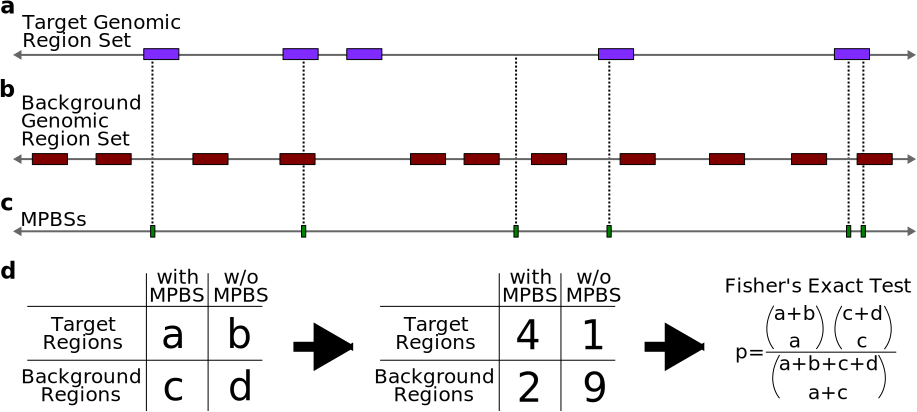
\includegraphics[width=0.99\textwidth]{gusmao_enrichment_analysis}
\caption[Transcription factor enrichment analysis]{\textbf{Transcription factor enrichment analysis.} (\textbf{a}) The target genomic region set is composed of the genomic regions under study. (\textbf{b}) The background genomic region set is composed of ``control'' genomic regions. It can be, for instance, random genomic regions in the same organism's genome. (\textbf{c}) Motif-predicted binding sites (motif-predicted binding sites) are created for a particular transcription factor in which we are interested in evaluating if enriched in the target genomic regions in contrast to the background genomic regions. (\textbf{d}) Based on the overlap between the target genomic region set, the background genomic region set and the motif-predicted binding sites for a particular transcription factor, we create a contingency table and evaluate the Fisher's exact test. The test's $p$-value gives an indication on the enrichment of the transcription factor at the target genomic regions.}
\label{fig:gusmao_enrichment_analysis}
\end{figure}


%%%%%%%%%%%%%%%%%%%%%%%%%%%%%%%%%%%%%%%%%%%%%%%%%%%%%%%%%%%%%%%%%%%%%
% Section: Case Study: Regulatory Network during Differentiation of Dendritic Cells
%%%%%%%%%%%%%%%%%%%%%%%%%%%%%%%%%%%%%%%%%%%%%%%%%%%%%%%%%%%%%%%%%%%%%
\subsection{Case Study: Regulatory Network during Differentiation of Dendritic Cells}
\label{sec:case.study.dendritic}

% Introduction - goals of study
Dendritic cells (DCs) are professional antigen presenting cells that develop from hematopoietic stem cells through successive steps of lineage commitment and differentiation. Multipotent progenitors (MPPs) are committed to DC restricted common DC progenitors (CDPs), which further differentiate into specific DC subsets: the classical DCs (cDCs) and plasmacytoid DCs (pDCs). The goal of this study is to understand the epigenetic and regulatory circuitry that determines the differentiation of MPPs to CDPs and CDPs to either cDCs or pDCs. The understanding of DC differentiation has impact on the further understanding of adaptive immune response.

% Here
In this study, ChIP-seq experiments were performed for several histone modifications, including H3K4me1. With the goal to capture the distal regulatory landscape of dendritic cell differentiation, we performed a transcription factor enrichment analysis using the footprints predicted with HINT on ChIP-seq for H3K4me1 -- a histone modification which indicates distal regulatory regions. The transcription factor enrichment analysis was performed using two different subsets of footprints. The H3K4me1 footprints that overlap with the transcription factor PU.1 ChIP-seq enriched regions (peaks) and the ones that do not overlap with PU.1. The rationale behind this analysis is that the transcription factor PU.1 is an important factor on the differentiation of dendritic cells (termed master regulator, given the fact that it initiates differentiation events). This analysis, which is a part of the study performed by Lin et al.~\cite{lin2015}, is presented as a case study for our computational footprinting framework in the next subsections.

%%%%%%%%%%%%%%%%%%%%%%%%%%%%%%%%%%%%%%%%%%%%%%%%%%%%%%%%%%%%%%%%%%%%%
% Section: Computational Footprinting
%%%%%%%%%%%%%%%%%%%%%%%%%%%%%%%%%%%%%%%%%%%%%%%%%%%%%%%%%%%%%%%%%%%%%
\subsubsection{Computational Footprinting}
\label{sec:cs1.computational.footprinting}

% Data
The ChIP-seq for histone modification H3K4me1 was performed in Zenke Lab and the data is available in GEO with accession number GSE57563~\cite{lin2015}. The short reads from the H3K4me1 ChIP-seq experiment were aligned to the mouse reference genome~\cite{encode2012} (NCBI37/mm9) using Bowtie~\cite{langmead2012}. To identify the H3K4me1 ChIP-seq enriched regions, the software MACS~\cite{zhang2008} version 1.4.2 was applied to the aligned reads.

% Computational Footprinting
Then we applied the histone-only HINT model (see ``Histone-only HMM'' in Section~\ref{sec:hmm.topology}). We followed the experimental settings as described in Chapter~\ref{cha:experiments}. Briefly, we extended the H3K4me1 enriched regions by $5,000$ bp to each side and applied our histone-only HMM model trained with H3K4me1 data from random genomic regions. Given the lower resolution of ChIP-seq data and the nature of the probabilistic model, footprints from H3K4me1 tend to span larger regions. Therefore, we further reduced the footprint predictions by considering only $250$ bp to the left (downstream) and right (upstream) of its center.

% Motif enrichment analysis
After the computational footprinting on H3K4me1 data, we used the footprint predictions to perform a transcription factor enrichment analysis (Section~\ref{sec:transcription.factor.enrichment.analysis}). We performed two different analyses. The first, considered H3K4me1 footprints that overlaps ChIP-seq peaks from the transcription factor PU.1 as the target genomic regions set. The second considered as target genomic regions set, the H3K4me1 footprints that do not overlap PU.1 binding sites. These two definitions of target genomic region sets were used for data on the four different cells being analyzed: MPPs, CDPs, cDCs and pDCs. In all cases, the background genomic region consisted of random genomic regions. The size of the background genomic region sets were $100$ times higher than the size of the target genomic region sets.

%%%%%%%%%%%%%%%%%%%%%%%%%%%%%%%%%%%%%%%%%%%%%%%%%%%%%%%%%%%%%%%%%%%%%
% Section: Results
%%%%%%%%%%%%%%%%%%%%%%%%%%%%%%%%%%%%%%%%%%%%%%%%%%%%%%%%%%%%%%%%%%%%%
\subsubsection{Results}
\label{sec:cs1.results}

% Intersection
The Figure~\ref{fig:lin_footprint_enrichment_s8}a shows the overlap between H3K4me1 footprints and PU.1 ChIP-seq enriched regions (peaks). We can observe different levels of overlap. As expected, higher overlap was found on more specialized cells (cDC; \approxy$68\%$ of H3K4me1 footprints overlap with PU.1 peaks) in contrast to more plastic cells (MPP; \approxy$23\%$ of H3K4me1 footprints overlap with PU.1 peak).

% Motif enrichment analysis result overview
As previously mentioned, we performed two motif enrichment analysis on the basis of the dendritic cell master regulator PU.1. The $p$-values from the transcription factor enrichment analyses are presented as a heatmap (see Figure~\ref{fig:lin_footprint_enrichment_s8}b and c). The enrichment is represented in a gray to blue scale. A gray heatmap entry represent no enrichment for the transcription factor represented in the row at the cell represented in the column. A blue heatmap entry represents evidence of enrichment. Enriched transcription factors were separated in different clusters (numbered I to VI) given their enrichment in different cells. The cluster entitled ``New'' represent the transcription factors that were found to be enriched in this analysis but were not found in a separate transcription factor enrichment analysis using only PU.1 peaks (without footprint information) as the target genomic region set (results not shown).

% Motif enrichment footprint + PU1
The first motif enrichment analysis results regard the experiments using H3K4me1 footprints that overlap PU.1 enriched regions as target genomic region set and random genomic regions as background genomic region set. The results of this motif enrichment analysis can be seen in Figure~\ref{fig:lin_footprint_enrichment_s8}b. As expected, since we are considering only footprints that overlap PU.1 peaks, the PU.1-like motifs (PU.1:SFPI1 and ETS1) are enriched in all cells. Nevertheless, it is interesting to observe that we captured some cell-specific PU.1 partners. In MPP we observed the binding of the pioneer PU.1 alongside evidence of CEBPA, KLF4 and RUNX1. The AP1-like transcription factors (FOS and JUN) and some IRF factors (IRF2, IRF4 and IRF5) appear to be cDC-specific. This means that these factors might have some role on the differentiation from CDP to cDC cell type. On the other hand, TCF factors (TCF3 and TCF4), EGR1, KLF4 and BHLHE40 appear to play a role in the differentiation from CDP to pDC cell type.

% Motif enrichment footprint - PU1
The second motif enrichment analysis results concerns the experiments using H3K4me1 footprints that do not overlap PU.1 enriched regions as target genomic region set and random genomic regions as background genomic region set. The results of this motif enrichment analysis can be seen in Figure~\ref{fig:lin_footprint_enrichment_s8}c. At first glance, we observe a lower number of enriched transcription factors. This is expected since the PU.1 transcription factor plays a major role in the differentiation of dendritic cells. The rationale of this analysis is to observe any evidence of PU.1-independent effects. IRF-like factors (IRF1, IRF8) and Stat1 appears to be associated to cDC differentiation. Interestingly, although these footprints do not overlap PU.1 enriched regions, we observed the PU.1 canonical motif in the cDC cell type (PU.1/SFPI1 and ETS1). Furthermore, as in the previous PU.1-centered enrichment analysis, the TCF factors (TCF3 and TCF4), EGR1, KLF4 and BHLHE40 are associated to pDC differentiation. It is interesting to observe the same enriched factors in both PU.1 enriched regions and PU.1 depleted regions for the pDC cell type, which stems from the same cell type (CDP) as the cDC, which contains the PU.1 canonical motif even in PU.1 depleted footprints.

% Figure - Dendritic cells footprint enrichment analysis results
\begin{figure}[h!]
\centering
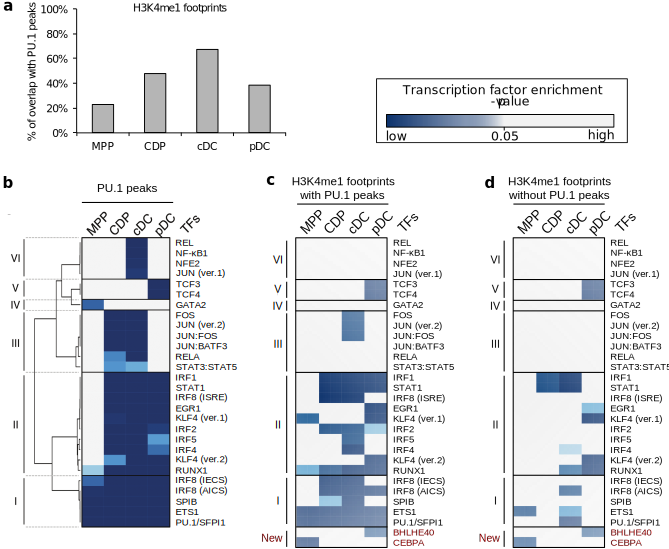
\includegraphics[width=0.99\textwidth]{lin_footprint_enrichment_s8}
\caption[Dendritic cells footprint enrichment analysis results]{\textbf{Dendritic cells footprint enrichment analysis results.} (\textbf{a}) The overlap of dendritic cell's master regulator transcription factor PU.1 ChIP-seq enriched regions with H3K4me1 footprints, which represent the distal regulatory regions, in the context of dendritic cell differentiation. (\textbf{b}) Heatmap depicts the enrichment of transcription factor motifs in MPP, CDP, cDC and pDC based on H3K4me1 footprints with PU.1 peaks. The $p$-values are plotted and color-coded using a continuous spectrum from gray ($p$-value > 0.05) to blue ($p$-value < 0.05). (\textbf{c}) The enrichment analysis of transcription factor motifs based on H3K4me1 footprints without PU.1 peaks, which identified a lower number of transcription factors. \emph{Source: Lin et al.}\cite{lin2015} (modified to fit thesis format and/or clarify key points).}
\label{fig:lin_footprint_enrichment_s8}
\end{figure}

% Conclusion
The results presented here demonstrate the power of computational footprinting coupled with \emph{post hoc} analyses (in this case, the transcription factor enrichment analysis). The H3K4me1 footprints represent distal regulatory regions and were shown to have a high overlap (\approxy$80\%$) with open chromatin regions. The H3K4me1 footprint predictions were used to search for transcription factors which act in conjunction with PU.1 master regulator or independently from the PU.1 master regulator. Such results, combined with other experimental data and knowledge from previous studies, were used to devise a regulatory network on the differentiation of dendritic cells. The complete results of these experiments can be found in Lin et al.~\cite{lin2015}.

%%%%%%%%%%%%%%%%%%%%%%%%%%%%%%%%%%%%%%%%%%%%%%%%%%%%%%%%%%%%%%%%%%%%%
% Section: Case Study: Multimodal Role of NF-kB during Intermmediate-Early Inflammatory Response
%%%%%%%%%%%%%%%%%%%%%%%%%%%%%%%%%%%%%%%%%%%%%%%%%%%%%%%%%%%%%%%%%%%%%
\subsection{Case Study: Multimodal Role of NF-$\kappa$B during Intermmediate-Early Inflammatory Response}
\label{sec:case.study.nfkb}

% Introduction - goals of study
Tumor necrosis factor alpha (TNF$\alpha$) acutely remodels the cell’s transcriptional program, but our understanding of how the activation of proinflammatory genes is achieved at the expense of the ongoing transcriptional program is far from complete. The transcription factor NF-$\kappa$B, the main driver of the inflammatory response, predominantly ``hijacks'' the regulatory machinery of the cell by binding already-active enhancers, more than half of which do not carry NF-$\kappa$B recognition motifs. The study performed by Kolovos et al.~\cite{kolovos2016} present evidence for a multimodal role of NF-$\kappa$B that satisfies the need for both transcriptional activation and suppression, and is linked with changes in the higher-order structure of regulated loci.

% Here
One of the analysis performed in Kolovos et al.~\cite{kolovos2016} regards a transcription factor enrichment analysis to understand the transcription factors associated to NF-$\kappa$B in regions that: either carry the NF-$\kappa$B DNA recognition motif or do not exhibit such motif. The analysis was performed on human Huvec cell type (umbilical vein/vascular endothelium). This analysis, which is a part of the study performed by Kolovos et al.~\cite{kolovos2016}, is presented as a case study for our computational footprinting framework in the next subsections.

%%%%%%%%%%%%%%%%%%%%%%%%%%%%%%%%%%%%%%%%%%%%%%%%%%%%%%%%%%%%%%%%%%%%%
% Section: Computational Footprinting
%%%%%%%%%%%%%%%%%%%%%%%%%%%%%%%%%%%%%%%%%%%%%%%%%%%%%%%%%%%%%%%%%%%%%
\subsubsection{Computational Footprinting}
\label{sec:cs2.computational.footprinting}

% Data
DNase-seq raw reads from Huvecs were obtained from ENCODE~\cite{encode2012}. The data is available in GEO with accession number GSM816646. The short reads from the DNase-seq experiment were aligned to the human reference genome~\cite{encode2012} (NCBI36/hg18) using Bowtie~\cite{langmead2012}. To identify the DNase I hypersensitivity regions (DNase-seq enriched regions), the software F-seq~\cite{boyle2008b} was applied to the aligned reads (using the procedure described in Section~\ref{sec:dnaseseq.enriched.regions}).

% Computational Footprinting
Then, we applied the DNase-only HINT model (see ``DNase-only HMM'' in Section~\ref{sec:hmm.topology}) to the DNase-seq data. We followed the experimental settings as described in Chapter~\ref{cha:experiments}. Briefly, we extended the DNase I hypersensitivity regions by $5,000$ bp to each side and applied our DNase-only HMM model trained with DNase-seq data from the Huvec experiments presented in this thesis (DNase-seq aligned to human reference genome NCBI37/hg19).

% Motif Enrichment Analysis
The resulting footprint predictions from the DNase-only HINT were separated in two categories. The footprint predictions that overlaps NF-$\kappa$B ChIP-seq enriched regions~\cite{papantonis2012} that: (1) carries the canonical NF-$\kappa$B motif and (2) do not carry such motif. Then we performed a transcription factor enrichment analysis in these two different conditions, considering the footprint predictions as our target genomic region set and random genomic regions as our background genomic region set. The size of the background genomic region sets were $100$ times higher than the size of the target genomic region sets.

%%%%%%%%%%%%%%%%%%%%%%%%%%%%%%%%%%%%%%%%%%%%%%%%%%%%%%%%%%%%%%%%%%%%%
% Section: Results
%%%%%%%%%%%%%%%%%%%%%%%%%%%%%%%%%%%%%%%%%%%%%%%%%%%%%%%%%%%%%%%%%%%%%
\subsubsection{Results}
\label{sec:cs2.results}

% Introduction
NF-$\kappa$B binding predominantly occurs at already-active (upon inflammation stimuli) distal regulatory regions called enhancers. These are mostly intragenic, display little overlap with CTCF-bound sites, and half carry the canonical motif or remain bound by NF-$\kappa$B at $60$ min after inflammatory stimulation. To obtain a more precise view of NF-$\kappa$B binding choices, we performed a transcription factor enrichment analysis on DNase-seq footprints. The analysis consists on comparing two different genomic region sets: (1) NF-$\kappa$B ChIP-seq enriched regions (peaks) at enhancer regions with the canonical NF-$\kappa$B motif and (2) NF-$\kappa$B ChIP-seq enriched regions (peaks) at enhancer regions without the canonical NF-$\kappa$B motif.

% Heatmap
The result of the transcription factor enrichment analysis can be seen in Figure~\ref{fig:kolovos_footprint_enrichment_2c}. We exhibit a heatmap that combines the two conditions tested. The color code is a gradient from blue (transcription factors enriched in NF-$\kappa$B peaks with motif) to white (no enrichment) to red (transcription factors enriched in NF-$\kappa$B peaks without motif).

% Results main
As expected, REL-like transcription factors (REL, RELA and NF-$\kappa$B1) are enriched in the NF-$\kappa$B peaks with canonical motif. Furthermore, the transcription factors KLF4, KLF7, ZNF281 and EGR1 appear to be significantly enriched in these regions. Among these factors, there are the TNF$\alpha$-induced REL, RELA, NF-$\kappa$B1, KLF7 and EGR1. On the other hand, we observe that the transcription factors  are significantly associated to NF-$\kappa$B-binding enhancer regions without the canonical NF-$\kappa$B motif. The only TNF$\alpha$-repressed transcription factor that appeared in our enrichment analysis -- SOX17 -- appears to be slightly associated to the regions without NF-$\kappa$B motif. The mechanisms behind these associated transcription factors and human inflammatory response are outside the scope of this thesis; however are further explored in Kolovos et al.~\cite{kolovos2016}.

% Further evidence
Briefly, the analysis shown that REL-like transcription factors (RELA and NF-$\kappa$B1) are markedly enriched at the NF-$\kappa$B peaks with canonical motif; whereas AP1-like transcription factors (JUN and FOS) appear to be enriched at the NF-$\kappa$B peaks without canonical motif. Further analyses show that the footprint enrichment analysis prediction is backed by ENCODE~\cite{encode2012} ChIP-seq data from Huvecs, where co-binding of NF-$\kappa$B and JUN/FOS (and to a lesser extent GATA2) was most prominent at enhancers without NF-$\kappa$B recognition sites.

% Figure - Huvec cells footprint enrichment analysis results
\begin{figure}[h!]
\centering
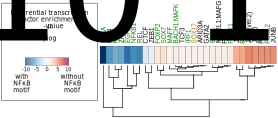
\includegraphics[width=0.99\textwidth]{kolovos_footprint_enrichment_2c}
\caption[Huvec cells footprint enrichment analysis results]{\textbf{Huvec cells footprint enrichment analysis results.} Heatmap showing the transcription factor enrichment analysis results at Huvec enhancer regions that overlap the footprints predicted with the DNase-only HINT model. The heatmap represents enrichment between ChIP-seq enriched regions with (blue) and without the canonical NF-$\kappa$B motif (red). Transcription factors induced or repressed by the inflammatory response factor TNF$\alpha$ are demarcated green and yellow, respectively. \emph{Source: Kolovos et al.}\cite{kolovos2016} (modified to fit thesis format and/or clarify key points).}
\label{fig:kolovos_footprint_enrichment_2c}
\end{figure}

% Conclusion
In contrast with the previous case study (Section~\ref{sec:case.study.dendritic}), where different cell types were being analyzed for the putative regulatory elements within their open chromatin regions; the analysis presented in this case study was based on two conditions which differed only in the presence/absence of the NF-$\kappa$B motif. In this case, the usage of DNase-seq alleviates much of the noise from intervening unbound sequence. The results presented in this section, combined with other experimental data, were used to understand the mechanisms behind hijacked enhancers and the regulatory role of NF-$\kappa$B in the human inflammatory mechanism. The complete results of these experiments can be found in Kolovos et al.~\cite{kolovos2016}.

